%%%%%%%%%%%%%%%%%%%%%%%%%%%%%%%%%%%%%%%%%%%%%%%%%%%%%%%%%%%%%%%%%%%%%%%%%%%%%%%%%%%%%%%%%%%%%%%%%%%%%%%%%%%%%%%%%%%%%%%%%%%%%%%%%%%%%%%%%%%%%%%%%%%%%%%%%%%%%%%%%%%%%%%%%%%%%%%%%%%%%%%%%%%%%%%%%%%%%%%%%%%%%%%%%%%%%%%%%%%%%%%%%%%
%%%%%%%%%%%%%%%%%%%%%%%%%%%%%%%%%%%%%%%%%%%%%%%%%%%%%%%%%%%%%%%%%%%%%%%%%%%%%%%%%%%%%%%%%%%%%%%%%%%%%%%%%%%%%%%%%%%%%%%%%%%%%%%%%%%%%%%%%%%%%%%%%%%%%%%%%%%%%%%%%%%%%%%%%%%%%%%%%%%%%%%%%%%%%%%%%%%%%%%%%%%%%%%%%%%%%%%%%%%%%%%%%%%
%%%%%%%%%%%%%%%%%%%%%%%%%%%%%%%%%%%%%%%%%%%%%%%%%%%%%%%%%%%%%%%%%%%%%%%%%%%%%%%%%%%%%%%%%%%%%%%%%%%%%%%%%%%%%%%%%%%%%%%%%%%%%%%%%%%%%%%%%%%%%%%%%%%%%%%%%%%%%%%%%%%%%%%%%%%%%%%%%%%%%%%%%%%%%%%%%%%%%%%%%%%%%%%%%%%%%%%%%%%%%%%%%%%
\chapter{The Large Hadron Collider}
In 2012, the peak luminosity was $7.7 \cdot 10^{33} \frac{1}{\text{cm}^2\,\text{s}}$.
The total integrated luminosity of $pp$~collisions over time recorded at the CMS experiment is shown in Fig.~\ref{fig:Lumi}.
The recording of events at the CMS experiment is devided into so-called ``runs'', where one run refers to a period of data taking in which the detector is working under stable conditions.
These runs are furthermore subdevided into ``luminosity blocks''.
They refer to short intervals of data taking ($<1\min$) in which the instantaneous luminosity is stable.
%%%%%%%%%%%%%%%%%%%%%%%%%%%%%%%%%%%%%%%%%%%%%%%%%%%%%%%%%%%%%%%%%%%%%%%%%%%%%%%%%%%%%%%%%%%%%%%%%%%%%%%%%%%%%%%%%%%%%%%%%%%%%%%%%%%%%%%%%%%%%%%%%%%%%%%%%%%%%%%%%%%%%%%%%%%%%%%%%%%%%%%%%%%%%%%%%%%%%%%%%%%%%%%%%%%%%%%%%%%%%%%%%%%
%%%%%%%%%%%%%%%%%%%%%%%%%%%%%%%%%%%%%%%%%%%%%%%%%%%%%%%%%%%%%%%%%%%%%%%%%%%%%%%%%%%%%%%%%%%%%%%%%%%%%%%%%%%%%%%%%%%%%%%%%%%%%%%%%%%%%%%%%%%%%%%%%%%%%%%%%%%%%%%%%%%%%%%%%%%%%%%%%%%%%%%%%%%%%%%%%%%%%%%%%%%%%%%%%%%%%%%%%%%%%%%%%%%
%%%%%%%%%%%%%%%%%%%%%%%%%%%%%%%%%%%%%%%%%%%%%%%%%%%%%%%%%%%%%%%%%%%%%%%%%%%%%%%%%%%%%%%%%%%%%%%%%%%%%%%%%%%%%%%%%%%%%%%%%%%%%%%%%%%%%%%%%%%%%%%%%%%%%%%%%%%%%%%%%%%%%%%%%%%%%%%%%%%%%%%%%%%%%%%%%%%%%%%%%%%%%%%%%%%%%%%%%%%%%%%%%%%
\FloatBarrier
\chapter{Event reconstruction and particle identification}


\section{The particle-flow algorithm}
\label{sec:PFalgorithm}
The particle-flow (PF) event description~\cite{CMS-PAS-PFT-09-001} aims at optimising particle identification and reconstruction by the usage of all sub-detector components of the CMS detector.
There are three main building bricks used for global event description: reconstructed charged-particle tracks, calorimeter clusters, and muon tracks.
The main requirements for these building bricks are a high reconstruction efficiency and a small fake rate.
Therefore, a special emphasis was put on developing a very efficient tracking algorithm (see Section~\ref{sec:ObjectReconstruction}) and a well performing calorimeter clustering algorithm~\cite{CMS-PAS-PFT-09-001}. 

The particle-flow algorithm proceeds as follows for each event (the description is based on~\cite{CMS-PAS-PFT-09-001}):
\begin{enumerate}
\item For each pair of detected building bricks, a ``link distance'' is calculated in order to quantify the quality of their link, \ie whether the two building bricks stem from the same particle. 
\item ``Blocks'' are produced from the building bricks that are linked together (with a typical number of one, two or three building bricks contained in a block) using different algorithms for different sets of building bricks (see~\cite{CMS-PAS-PFT-09-001} for detailed information about these algorithms).
      Blocks comprise either charged-particle tracks and calorimeter clusters, or several calorimeter clusters, or a charged-particle track in the tracker and a muon track in the muon system.
      The latter is called a global muon.
\item For each block the following steps are performed:
\begin{enumerate}
\item Each global muon where the \pt measured in both sub-detectors is compatible with the  \pt  measurement in the tracker is defined as a particle-flow muon and the track in both sub-detectors is removed from the block.
\item Next, electrons are reconstructed and identified using tracker hits and ECAL clusters. 
      For an identified particle-flow electron, the corresponding tracker hits and the ECAL clusters (including energy deposits from Bremsstrahlung photons) are removed from the block. 
\item Tighter track quality criteria are applied.
\item The compatibility of the remaining ECAL and HCAL energy deposits to the transverse momentum of the reconstructed tracks within a block is checked. 
      This allows for the identification of particle-flow charged hadrons with a momentum estimate using tracker and calorimeter information. 
      If the energy deposits in the ECAL or HCAL are much larger than the corresponding track \pt, the signature is identified as a particle-flow photon or particle-flow neutral hadron, respectively. 
      All ECAL and HCAL clusters used for the identification as well as the reconstructed tracks are removed from the block.
\item Finally, the remaining ECAL and HCAL clusters (which are all not linked to any other building block) are identified as particle-flow photons or particle-flow neutral hadrons, respectively.
\end{enumerate}
\end{enumerate}
For the final identification of particles and other objects further reconstruction criteria are applied (see Section~\ref{sec:ObjectReconstruction}).

\section{Object reconstruction}
\label{sec:ObjectReconstruction}
In this section, an overview of the required criteria for the identification of particles and other physics objects is given.

\subsection{Reconstruction of primary vertices} 
\label{sec:VertexReconstruction}
The reconstruction of primary vertices (PVs) is important in order to determine the location of the interaction point and to get an estimate of the corresponding uncertainty.
At the CMS experiment, the reconstruction of vertices proceeds as follows~\cite{bib:CMS:tracking_8TeV}:
First, a track selection is performed which depends on the number of hits in the tracker, on the significance of the transverse distance to the beam spot ($|d_0^{\text{BS}}|/\delta d_0$), and the normalised $\chi^2$ of the track fit (see the subsequent Section~\ref{subsec:TrackReconstruction} for more information on the track reconstruction algorithms).
All selected tracks are afterwards clustered to several vertices based on their point of closest approach in $z$-direction to the beam spot.
The clustering first identifies candidate vertices using a so-called deterministic annealing (DA) algorithm~\cite{bib:VertexReconstruction_DA}.
Subsequently, the candidate vertices are evaluated with the adaptive vertex fitter~\cite{bib:VertexReconstruction_AVF}, which estimates the location of the vertices as well as performance parameters of the fit.
A weight is assigned to each track that is close to one in case for a good compatibility and close to zero for a bad compatibility with the vertex.
The track with the largest sum of all squared track transverse momenta, $\sum \pt^2$, is referred to as the primary vertex. 
All other vertices during a bunch-crossing are so-called pileup interactions.

Further quality criteria of the primary vertex are required in the search for highly ionising, short tracks (Part~\ref{part:analysis}) and the measurement of the jet transverse-momentum resolution (Part~\ref{part:resolution}).
For this purpose, the ``number of degrees of freedom'' of the primary vertex is introduced: 
\begin{equation}
n_{\text{dof}} = -3 + 2 \sum_{\text{tracks}} w_i.
\end{equation}
The requirement of a well reconstructed primary vertex is  $n_{\text{dof}}>4$.
Furthermore, the vertex is required to be within 24\cm in $z$- and 2\cm in $r$-direction with respect to the nominal interaction point.


\subsection{Reconstruction of tracks}
\label{subsec:TrackReconstruction}
The reconstruction of tracks aims at linking several hits in the tracking system to one reconstructed track that matches the original trajectory of the particle with a high probability.
With the track reconstruction, an estimate of the particle momentum as well as its position can be achieved.
Track reconstruction is challenging because the large number of hits\footnote{At design luminosity around 1000 charged particles are expected to traverse the tracker in each bunch-crossing~\cite{bib:CMS:tracking_8TeV}}, especially in the layers close to the interaction vertex, leads to a high combinatorial complexity. 
In the following, an overview of the tracking algorithm used at CMS is given.
It is based on~\cite{bib:CMS:tracking_8TeV} and the reader is referred to this reference for more information on the reconstruction of tracks at CMS.\\

The tracking software used at CMS is usually referred to as the Combinatorial Track Finder (CTF).
It it based on the so-called combinatorial Kalman filter~\cite{bib:TrackAlgorithm_1989,bib:TrackAlgorithm_1990,bib:TrackAlgorithm_1997} which in turn is based on the Kalman filter~\cite{bib:KalmanFilter_1987}.
The Kalman filter is an algorithm that allows for the estimation of parameters of interest based on a set of observations that are subject to noise or other inaccuracies.
It is mathematically equivalent to a global least square minimisation for linear models with Gaussian noise.

The basic idea of the tracking algorithm at CMS is to avoid applying the combinatorial Kalman filter on all hits in one step by using an iterative procedure (called iterative tracking).
A reduction of complexity can be achieved by first reconstructing tracks that are easy to identify because of \eg a relatively high \pt. 
These tracks are removed afterwards and the remaining tracker hits are subject to further reconstruction iterations.
The following iterations are performed (these steps refer to the setting from May to August in 2011 but are in their basic structure retained in the year 2012):
\begin{itemize}
\item Iteration 0: Tracks near the \pp-interaction point that have three pixel hits and a $\pt>0.8\gev$ are reconstructed.
\item Iteration 1: Tracks with only two pixel hits and $\pt>0.8\gev$ are reconstructed. 
\item Iteration 2: Low \pt tracks from the \pp-interaction point are reconstructed.
\item Iteration 3-5: Reconstruction of tracks that are not originating from the primary vertex or that were not found by previous iterations.
\end{itemize}
Within these iterations, the reconstruction is subdivided into four different steps:
\begin{itemize}
\item Seed generation: Only 2-3 hits are used to define track candidates.
\item Extrapolation: Based on the expected flight path, additional hits are assigned to the candidate track using a combinatorial Kalman filter.
\item Track fitting: With the usage of the Kalman filter and a smoother, the trajectory is fitted in order to estimate the track parameters.
\item Setting of quality flags: Quality flags are assigned to all tracks and tracks that fail certain quality criteria are discarded.\\
\end{itemize}
%The configuration of the first and the fourth step differs across the different iterations.  

A special task when reconstruction tracks consists of the suppression of fake tracks, \ie tracks that are not associated with a charged particle.
Therefore, the requirement of fulfilling certain quality criteria (fourth step) is crucial to substantially reduce the contamination of fake tracks.
 For this purpose, requirements on the following variables are imposed (the values of the parameters $\alpha$ and $\beta$ vary across iterations):
\begin{itemize}
\item A minimum number of layers in which the track has an associated hit.
\item A minimum number of layers in which the track has an associated 3D hit\footnote{A 3D hit refers to a measurement that provides 3D position information, such as a pixel hit or a strip hit in a stereo module.}.
\item A maximum number of layers in which the track has no associated hit.
\item A high quality of the trajectory fit: $\chi^2/\text{ndof} < \alpha_0 N_{\text{layers}}$.
\item A low transverse impact parameter significance:  $|d_0^{\text{BS}}|/\delta d_0 < \left( \alpha_3 N_{\text{layers}} \right)^{\beta}$,\\
\hspace*{231pt}                                        $|d_0^{\text{BS}}|/\sigma_{d_0} \left(\pt\right) < \left( \alpha_1 N_{\text{layers}} \right)^{\beta}$.
\item A low longitudinal impact parameter significance: $|z_0^{\text{PV}}|/\delta z_0 < \left( \alpha_4 N_{\text{layers}} \right)^{\beta}$\\
\hspace*{240pt}                                         $|z_0^{\text{PV}}|/\sigma_{z_0} \left(\pt,\eta\right) < \left( \alpha_2 N_{\text{layers}} \right)^{\beta}$.
\end{itemize}
The variable $d_0^{\text{BS}}$ is the distance of the track to the centre of the beam spot in the transverse plane to the beam line and $z_0^{\text{PV}}$ is the distance along the beam line to the closest pixel.
The variables $\delta d_0$ and $\delta z_0$ are the uncertainties on the distance (impact) parameters and $\sigma$ is the standard deviation corresponding to the length of the beam spot in z-direction.




\subsection{Reconstruction of photons}
\label{subsec:PhotonReconstruction}
The following description of the photon reconstruction is based on~\cite{bib:CMS:PhotonIdentification_8TeV}, where also a more detailed explanation of the photon reconstruction algorithms can be found.

Photons are reconstructed from energy deposits in the ECAL.
The clustering algorithms of the ECAL energy deposits do not differentiate between electrons and photons.
Thus, they are the same as used for electron identification (Section~\ref{subsec:ElectronReconstruction}).
So-called ``superclusters'' are formed from a ``seed crystal'' which has an energy deposit greater than all of its neighbouring crystals and above a certain threshold.
In the barrel region a so-called ``hybrid'' algorithm is used which proceeds by adding in $\phi$ direction fixed arrays of $5 \times 1$ crystals in $\eta \times \phi$ if their energy deposits are larger than a certain minimal energy.
In the endcap region, the so-called ``multi $5 \times 5$'' clustering algorithm is used.
It proceeds by adding fixed arrays of $5 \times 5$ crystals if their energy exceeds a certain threshold.
These clustering procedures collect energy from radiating electrons as well as converted photons.

After the clustering the measured energy in a supercluster is subject to an energy correction procedure~\cite{bib:CMS:PhotonIdentification_8TeV}.
The energy estimate is finally based on the variable $R_9$.
It is the ratio of the energy deposit within a $3\times 3$ array of crystals around the seed crystal divided by the total energy in the supercluster.
This variable nicely discriminates between converted and unconverted photons as can be seen in Fig.~\ref{fig:PhotonR9}.
\begin{figure}[!t]
  \centering
      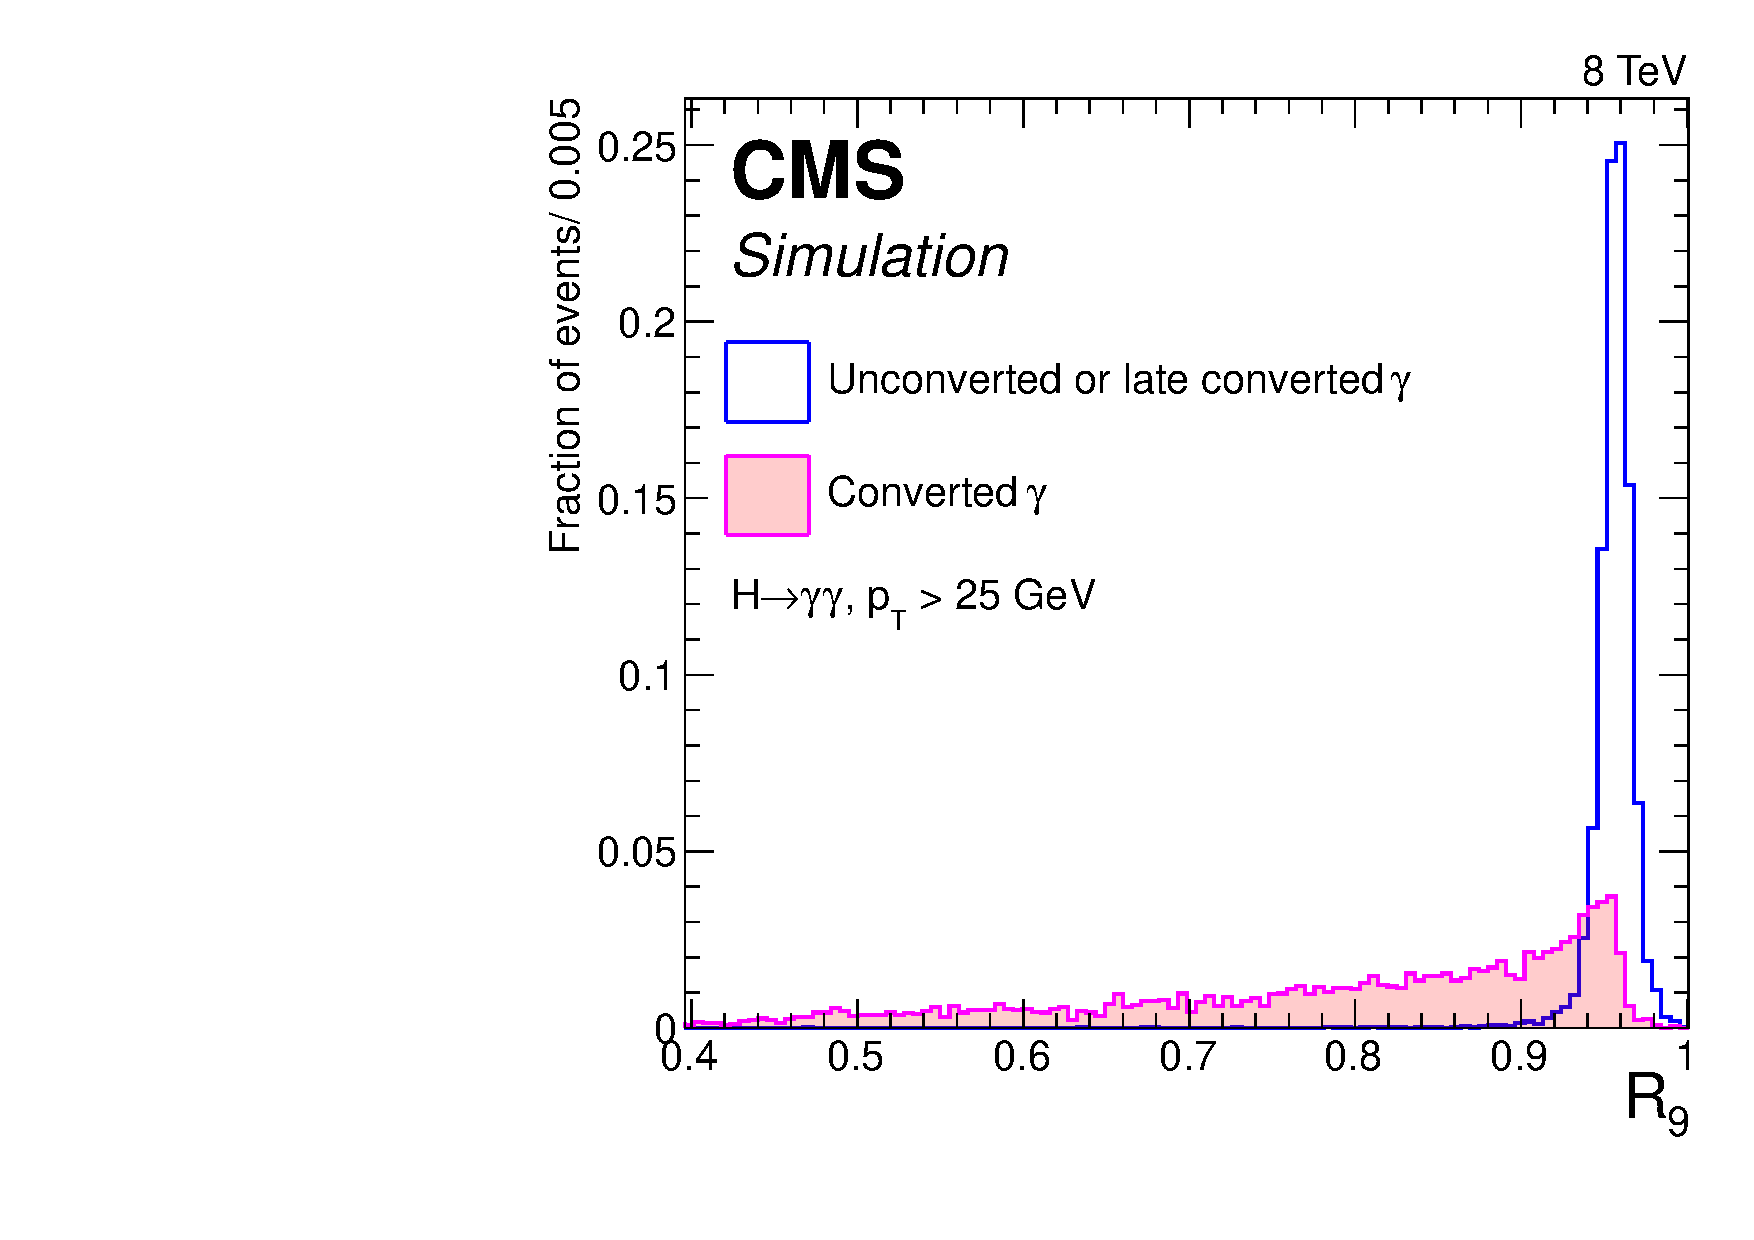
\includegraphics[width=0.50\textwidth]{figures/experiment/ObjectReconstruction/convUnconvR9Linear}
      \caption{Normalised distribution of the $R_9$ variable for converted and unconverted (or late converted) photons. Taken from~\cite{bib:CMS:PhotonIdentification_8TeV}}  
  \label{fig:PhotonR9}
\end{figure}
The energy spread is wider for converted photons than for unconverted photons.
Thus, the energy is estimated as the sum of energy deposits in the superclusters for converted photons ($R_9<0.94$ in the barrel and $R_9<0.94$ in the endcap region) and as the sum of energy deposits in the $5\times5$ crystal matrix for the unconverted photons.



